\documentclass[%
reprint,
amsmath,amssymb,
aps,
]{revtex4-1}
\usepackage{graphicx}% Include figure files
\usepackage{dcolumn}% Align table columns on decimal point
\usepackage{bm}% bold math
\usepackage[utf8]{inputenc}
\usepackage{listings}
\usepackage{amsmath}
\usepackage{physics}
\usepackage{caption}
\usepackage{subfig}
\usepackage{float}
\usepackage{stfloats}

\makeatletter
\newcommand*{\rom}[1]{\expandafter\@slowromancap\romannumeral #1@}
\makeatother

\begin{document}
\title{Eigenvalue problems}
\author{Torstein S. Ølberg, Ada M. Veddegjerde and Oline A. Ranum}
\affiliation{%
 \textnormal{Universitetet i Oslo, Institutt for fysikk}\\
 olinear@student.matnat.uio.no : torsteol@student.matnat.uio.no
}
\date{\today}


\begin{abstract}
	The following experiment was undertaken as
\end{abstract}
\maketitle

\section*{Introduction}


\section*{Theory}
\subsection{The eigenvalue problem} \noindent 
Given a matrix A of dimension N, the eigenvalues of A are defined through the equation
\begin{equation}\label{eigenval}
	\mathbf{Ax}^{(v)} = \lambda^{(v)}\mathbf{x}^{(v)}
\end{equation}
where $\lambda^{(v)}$ is the eigenvalues and $\mathbf{x}^{(v)}$ the corresponding eigenvectors. The eigenvalue problem is equivalent to a set of $n$ equations with $n$ unknowns 
\begin{align*}
	a_{11}x_1 + a_{12}x_2 +\dots + a_{1n}x_n = \lambda x_1 \\a_{21}x_1 + a_{22}x_2 +\dots + a_{2n}x_n = \lambda x_2 \\ \dots \hspace{2mm} \dots \\
	a_{n1}x_1 + a_{n2}x_2 +\dots + a_{nn}x_n = \lambda x_n \\
\end{align*}
Such a set of equations can be solved by moving all factors to the left hand side and then take the determinant of the system. This is often considered to be a highly inefficient way of solving the problem for large values of n. Therefore, alternative numerical solutions have been developed for solving such systems. 

\subsection{Eigensystem solvers} \noindent 
In the case that the matrix $\mathbf{A}$ is on a diagonal form, the eigenvalues of $\mathbf{A}$ is the diagonal elements. Similarity transformations provides one way of transforming a $N\times N$ matrix $\mathbf{A}$ into a diagonal matrix $\mathbf{D}$. In general, a similarity transformation $\mathbf{S}$ is a conformal mapping yielding the transformation matrix $\mathbf{B}$ on the form
\begin{equation*}
	\mathbf{B} = \mathbf{SAS^{-1}}
\end{equation*}
\noindent In the case that the matrix $\mathbf{A}$ is both symmetric and real, this is equivalent to  

\begin{equation*} \label{eq2}
\mathbf{B} = \mathbf{S}^T\mathbf{A}\mathbf{S}, \hspace{3mm} \textnormal{where} \hspace{3mm} \mathbf{S}^T\mathbf{S} = \mathbf{S}^{-1}\mathbf{S} = \mathbf{I}
\end{equation*}
By choosing the correct transformation it is possible to preform a series of similarity transformations on $\mathbf{A}$ in order to reduce it to a diagonal form. That is, by subsequently applying a similarity transform so that 
\begin{equation*}
\mathbf{D} = \mathbf{S}_N^T...\mathbf{S}_1^T\mathbf{A}\mathbf{S}_1...\mathbf{S}_N 
\end{equation*}
where 
\begin{equation*}
	\mathbf{D} = \begin{bmatrix}
	\lambda_1 & 0 & 0 & \dots & 0 \\
	0 & \lambda_2 & 0 & \dots & 0 \\
	\vdots & \vdots & \vdots &\vdots&\vdots\\
	0 & 0 & 0 &\dots & \lambda_n
	\end{bmatrix}
\end{equation*}
where $\lambda_i$ are the eigenvalues of $\mathbf{A}$. A similarity transformation on $\mathbf{A}$ yields a matrix with the same eigenvalues, but in general different eigenvectors. This is the concept underlying the method known as Jacobi's method [M. Jensen, 2015].

\subsubsection*{Jacobi's method}  \noindent 
Jacobi's method exploits similarity transformations to preform a rotation of the plane. The method transforms a matrix into a diagonal or tridiagonal form using Housholder's algorithm. In this case the matrix considered is an $n\times n$ orthogonal transformation matrix on the form \vspace{1mm}
\begin{equation*}
\mathbf{S} = \begin{bmatrix}
1 & 0  & \dots & 0 &\vdots &0 \\
0 & 1  & \dots & 0 & \vdots & 0 \\
\vdots & \vdots &\vdots&\vdots&\vdots&\vdots\\
0 & 0 & \cos{\theta} & 0 &\vdots & \sin{\theta} \\
0  & 0 & 0 & 1 &\vdots & 0 \\
 \vdots & \vdots &\vdots&\vdots&\vdots&\vdots\\
 0 & 0 &\dots & -\sin{\theta} & \vdots & \cos{\theta}
\end{bmatrix}
\end{equation*}\vspace{1mm}
\noindent 
This matrix makes a plane rotation of an angle $\theta$ in the Euclidean n-dimensional space. The similarity matrix is defined through the quantities $\tan\theta = t= s/c$, with $s=\sin\theta$ and $c=\cos\theta$ and
\begin{equation*}\cot 2\theta=\tau = \frac{a_{ll}-a_{kk}}{2a_{kl}}.
\end{equation*}
where $a_{kl}$ should be the largest off-diagonal matrix element in order to ensure that all other off-diagonal elements converges towards zero during the sequential transformations. The identity $\cot 2\theta=1/2(\cot \theta-\tan\theta)$ leads to the quadratic equation
\begin{equation*}
t^2+2\tau t-1= 0,
\end{equation*}
resulting in
\begin{equation*}
t = -\tau \pm \sqrt{1+\tau^2},
\end{equation*}
One chooses the sign that minimizes t. Then $c$ and $s$ are easily obtained via
\begin{equation}\label{sc}
c = \frac{1}{\sqrt{1+t^2}} \hspace{5mm}  \textnormal{and} \hspace{5mm} s=tc
\end{equation}  \vspace{2mm}
\noindent
This leads to the following equations of transformation \vspace{1mm}
\begin{align*}
&b_{ii} = a_{ii} \hspace{49mm} i\not=k & i\not=l\\
&b_{ik} = a_{ik}\cos\theta -a_{il}\sin\theta \hspace{25mm} i\not=k & i\not=l \\
&b_{il}  = a_{il}\cos\theta -a_{ik}\sin\theta \hspace{26mm} i\not=k & i\not=l\\ &&\\
&b_{kk} = a_{kk}\cos^2\theta -2a_{kl}\cos\theta\sin\theta +a_{ll}\sin^2\theta&\\
&b_{ll} = a_{ll}\cos^2\theta -2a_{kl}\cos\theta\sin\theta +a_{kk}\sin^2\theta& \\
&b_{kl} = (a_{kk}-a_{ll})\cos\theta\sin\theta+a_{kl}(\cos^2\theta -\sin^2\theta)& \\
\end{align*}\begin{equation}
	\label{jacobimethod}
\end{equation}

\subsection{Unitary transformations} \noindent 
It can be showed that a unitary transformation is a transformation that preserves the orthogonality and inner product. Given a basis of vectors $\vec{v_i}$ ,
\begin{equation*}
	\mathbf{v}_i = \begin{bmatrix} v_{i1} \\ \dots \\ \dots \\v_{in} \end{bmatrix}
\end{equation*}
where the basis is orthogonal 
\begin{equation*}
	\mathbf{v}_j^T\mathbf{v}_i = \delta_{ij}
\end{equation*}
Given the unitary transformation 
\begin{equation*}
	\mathbf{w}_i=\mathbf{U}\mathbf{v}_i
\end{equation*}
It can be shown that the transformation preserves orthogonality
\begin{align*}
	\mathbf{w}=\mathbf{U}\mathbf{v} &\implies \mathbf{w}^T=\mathbf{v}^T\mathbf{U}^T \\ &\implies \mathbf{w}^T\mathbf{w} = \mathbf{v}^T\mathbf{U}^T\mathbf{U}\mathbf{v} = \mathbf{v}^T\mathbf{v} = \delta
\end{align*}
To show that it preserves the inner product we define 
\begin{align*}
	\mathbf{a} &= U\mathbf{b} \\
	\rightarrow \mathbf{a}^T &= \mathbf{b}^TU^T \\
	&\textnormal{We then take the inner product:} \\
	 \mathbf{a}^T\mathbf{w} &= \mathbf{b}^TU^TU\mathbf{v} = \mathbf{b}^T\mathbf{v}
\end{align*}
Where we have showed that the unitary transformation does not affect the inner product. 


\subsection{The buckeling beam problem} \noindent 
The classical harmonic oscillator potential is described by the following equation of motion
\begin{equation}\label{evp}
\frac{d^2 u(x)}{dx^2} = -k u(x)
\end{equation}
where $u(x)$ is the vertical displacement of the system in the $y$ direction. This general equation is the foundation for a large set of physical systems, that often can be solved using numerical eigenvalue solvers. For instance a spring force or the buckling beam problem. \\ \indent 
 In the case of the buckling beam $k = F/\gamma$, where F is the force applied at the end of the beam in the direction towards the origin, and $\gamma$ is a constant defined by inherent properties of the beam. This system will here assume the Dirichlet boundary conditions
 \begin{equation*}
 	u(0) = u(L) = 0
 \end{equation*}
where L is the length of the beam. If one defines the dimensionless variable $\rho = x/L$, one can reorder the equation into
\begin{equation}\label{bb}
\frac{d^2 u(\rho)}{d\rho^2} = -\frac{FL^2}{R} u(\rho)=-\lambda u(\rho)
\end{equation}
This equation becomes an eigenvalue problem when discretized, on the form equation \ref{eigenval}. Applying a Taylor approximation to the second derivative of the differential equation, a discretized variant of the equation can be expressed as
\begin{equation}\label{eqdis}
-\frac{u_{i+1} -2u_i +u_{i-1} }{h^2}  = \lambda u_i
\end{equation}


\subsubsection{The analytical solution of a tridiagonal matrix} \noindent 
Systems on the form of equation \ref{eqdis} is known as a Toeplitz tridiagonal matrix, and has analytical eigenpairs. These eigenvalues are given by the formula
\begin{equation}\label{analytical}
\lambda_j = d+2a\cos{(\frac{j\pi}{N+1})} \hspace{0.1cm} j=1,2,\dots N-1
\end{equation}



\subsection{The Quantum Harmonic Oscillator} \noindent 
Another famous harmonic oscillator is the description of electron systems. For a system assuming spherical symmetry, the radial part of the Schroedinger equation for one electron reads
\begin{equation*}
-\frac{\hbar^2}{2 m} \left ( \frac{1}{r^2} \frac{d}{dr} r^2
\frac{d}{dr} - \frac{l (l + 1)}{r^2} \right )R(r) 
+ V(r) R(r) = E R(r).
\end{equation*}
where V(r) is set to be the harmonic oscillator potential 
\begin{equation*}
	V(r) = \dfrac{1}{2}kr^2 = \dfrac{1}{2}m\omega^2r^2
\end{equation*}
E is the energy of the harmonic oscillator in three dimensions, and given the oscillator frequency $\omega$ the energy eigenvalues correspond to 
\begin{equation*}
E_{nl}=  \hbar \omega \left(2n+l+\frac{3}{2}\right),
\end{equation*}
with energy level $n=0,1,2,\dots$ and the orbital momentum $l=0,1,2,\dots$ of the electron. Though the usual substitution $R(r) \rightarrow u(r)/r$ and introduction of the dimensionless variable $\rho = r/\alpha$, $\alpha$ is a constant with dimension length, we get

\begin{equation*}
-\frac{\hbar^2}{2 m \alpha^2} \frac{d^2}{d\rho^2} u(\rho) 
+ \left ( V(\rho) + \frac{l (l + 1)}{\rho^2}
\frac{\hbar^2}{2 m\alpha^2} \right ) u(\rho)  = E u(\rho)
\end{equation*}
The boundary condition is given by the Dirichlet conditions, and the equation is further reduced by inserting the potential with l = 0. After some shuffling of constants one gets the equation  
\begin{equation*}
-\frac{d^2}{d\rho^2} u(\rho) 
+ \frac{mk}{\hbar^2} \alpha^4\rho^2u(\rho)  = \frac{2m\alpha^2}{\hbar^2}E u(\rho) .
\end{equation*}
Where $\alpha$ is fixed to be 
\begin{equation*}
\alpha = \left(\frac{\hbar^2}{mk}\right)^{1/4}
\end{equation*}
This comes together to yield the energy eigenvalues 
\begin{equation*}
\lambda = \frac{2m\alpha^2}{\hbar^2}E,
\end{equation*}
and the Schroedinger's equation can be expressed as
\begin{equation}\label{qho}
-\frac{d^2}{d\rho^2} u(\rho) + \rho^2u(\rho)  = \lambda u(\rho)
\end{equation}
See any introductory book on quantum mechanics for for further details. [Griffiths, 2018]. 

\subsubsection{The discretized quantum harmonic oscillator}
Looking to the discretization of equation \ref{eqdis}, we see that it can be expanded to also cover this problem by a small modification. By including the electron-electron potential we now write 
\begin{equation}\label{eqho2}
\begin{aligned}
	-\frac{u_{i+1} -2u_i +u_{i-1}}{h^2}+\rho_i^2u_i \\=-\frac{u_{i+1} -2u_i +u_{i-1} }{h^2}+V_iu_i  = \lambda u_i
\end{aligned}
\end{equation}
where $V_i=\rho_i^2$ is the harmonic oscillator potential. To solve this problem numerically one sets all diagonal elements to 
\begin{equation}\label{hoeq3}
d_i=\frac{2}{h^2}+V_i
\end{equation}
and set all non-diagonal matrix elements to
\begin{equation}\label{hoeq4}
e_i=-\frac{1}{h^2}
\end{equation}
By this definition the Schrödinger equation can be described as
\begin{equation*}
d_iu_i+e_{i-1}u_{i-1}+e_{i+1}u_{i+1}  = \lambda u_i,
\end{equation*}
where $u_i$ is unknown. This yields the eigenvalue problem
\begin{equation}\label{evho}
\begin{bmatrix}d_0 & e_0 & 0   & 0    & \dots  &0     & 0 \\
e_1 & d_1 & e_1 & 0    & \dots  &0     &0 \\
0   & e_2 & d_2 & e_2  &0       &\dots & 0\\
\dots  & \dots & \dots & \dots  &\dots      &\dots & \dots\\
0   & \dots & \dots & \dots  &\dots  e_{N-1}     &d_{N-1} & e_{N-1}\\
0   & \dots & \dots & \dots  &\dots       &e_{N} & d_{N}
\end{bmatrix}  \begin{bmatrix} u_{0} \\
u_{1} \\
\dots\\ \dots\\ \dots\\
u_{N}
\end{bmatrix}=\lambda \begin{bmatrix} u_{0} \\
u_{1} \\
\dots\\ \dots\\ \dots\\
u_{N}
\end{bmatrix}
\end{equation}

\subsubsection{Quantum harmonic oscillator with two electrons} \noindent 
The two electron system can be described in a similar way, but one the repulsive Coulomb interaction must be included as well. The single-single electron equation is more precisely described as
\begin{equation*}
    -\frac{\hbar^2}{2m}\frac{d^2}{dr^2}u(r)+\frac{1}{2}kr^2u(r) = E^{(1)}u(r),
\end{equation*}
here $E^{(1)}$ stands for the energy with only one electron. For two electrons, with no repulsive Coloumb interaction for now, the Schroedinger equation becomes
\begin{equation*}
    \left(-\frac{\hbar^2}{2m}\frac{d^2}{dr^2_1}-\frac{\hbar^2}{2m}\frac{d^2}{dr^2_2}+\frac{1}{2}kr^2_1+\frac{1}{2}kr^2_2\right)u(r_1,r_2) = E^{(2)}u(r_1,r_2).
\end{equation*}
This equation can easily be expanded to a two-electron wave function $u(r_1,r_2)$ with energy $E^{(2)}$.\par
Since there is no interaction the solution will be of a closed form, that means it can be written as the product of two single-electron wave functions.\par
By introducing two new coordinates, the relative coordinate $\bm{r}=\bm{r}_1-\bm{r}_2$ and the center-of-mass coordinate $\bm{R}=1/2(\bm{r}_1+\bm{r}_2)$, the radial Schroedinger equation reads
\begin{equation*}
    \left(-\frac{\hbar^2}{m}\frac{d^2}{dr^2}-\frac{\hbar^2}{4m}\frac{d^2}{dR^2}+\frac{1}{4}kr^2+kR^2\right)u(r,R) = E^{(2)}u(r,R).
\end{equation*}
\par The equation can be separated into $r$ and $R$ via the ansatz for the wave function $u(r,R)=\psi(r)\phi(R)$ and the energy is given by the sum of the relative energy and the center-of-mass energy. Therefore the equation can be formulated as
\begin{equation*}
    E^{(2)} = E_r+E_R.
\end{equation*}
\par To include the repulsive Coulomb interaction between two electrons one can add the term
\begin{equation*}
    V(r_1,r_2) = \frac{\beta e^2}{|\bm{r}_1-\bm{r}_2|} = \frac{\beta e^2}{r},
\end{equation*}
with $\beta e^2=1.44 eVnm$.
\par Now the r-dependent Schroedinger equation becomes 
\begin{equation*}
    \left(-\frac{\hbar^2}{m}\frac{d^2}{dr^2}+\frac{1}{4}kr^2+\frac{\beta e^2}{r}\right)\psi(r) = E_r\psi(r)
\end{equation*}
This equation is similar to the one of the one electron case, and again the dimensionless variable $\rho = r/\alpha$ can be introduced. By repeating the same
steps as before, the equation reads
\begin{equation*}
  -\frac{d^2}{d\rho^2} \psi(\rho) 
       + \frac{1}{4}\frac{mk}{\hbar^2} \alpha^4\rho^2\psi(\rho)+\frac{m\alpha \beta e^2}{\rho\hbar^2}\psi(\rho)  = 
\frac{m\alpha^2}{\hbar^2}E_r \psi(\rho).
\end{equation*}
In order to make the equation as similar to that in \ref{qho}
as possible, new 'frequency' can be defined as

\begin{equation*}
\omega_r^2=\frac{1}{4}\frac{mk}{\hbar^2} \alpha^4,
\end{equation*}
Then constant $\alpha$ can be fixed by requiring

\begin{equation*}
\frac{m\alpha \beta e^2}{\hbar^2}=1
\end{equation*}
or

\begin{equation*}
\alpha = \frac{\hbar^2}{m\beta e^2}.
\end{equation*}
Defining

\begin{equation*}
\lambda = \frac{m\alpha^2}{\hbar^2}E,
\end{equation*}
The Schroedinger's equation can be expressed as
\begin{equation}\label{qho2}
  -\frac{d^2}{d\rho^2} \psi(\rho) + \omega_r^2\rho^2\psi(\rho) +\frac{1}{\rho} = \lambda \psi(\rho).
\end{equation}


\subsection{The Frobenius norm} \noindent 
The Frobenius norm is a matrix norm defined as the square root of the sum of the absolute squares of its elements 
\begin{equation}\label{forb}
\parallel A \parallel_F^2 = \parallel B \parallel_F^2 = \sum_{ij} \abs{a_{ij}}^2 = \sum_{ij} \abs{b_{ij}}^2
\end{equation}
The Frobenius norm is conserved under orthogonal/unitary transformations. 
\newpage 
\section*{Method}
\subsection*{M\rom{1}. Jacobi's method for solving the buckling beam problem}
\noindent We initialize a tridiagonal Toplitz matrix on the form of equation \ref{eqdis}, in order to solve the buckling beam problem of equation \ref{bb}. Next, we implement Jacobi's method based on the block of equation given in equation set \ref{jacobimethod}, where $c = \cos{\theta}$ and $s = sin{\theta}$ are defined as in equation \ref{sc}. We apply Dirichlet boundary conditions and set a threshold for the transformation-series on the Fobernius norm of equation \ref{forb} of all off-diagonal elements. The sum must be smaller than $10^{-10}$ for all off-diagonal elements to be considered to be zero. We then state that the transformed matrix is on a diagonal form, and we read the eigenvalues of the matrix $\hat{D}$ across the diagonal. \\ \indent 
When we have the eigenvalues produced by the Jacobi's method, we go on to compare them with the analytical eigenvalues of equation \ref{analytical}. To evaluate the efficiency of Jacobi's method in regards to other known possibilities for finding the eigenvalues, we implement the Armadillo \textit{eig$\_$sym} function. We compare both the time of both methods and the accuracy in regards to the analytical solutions. We furthermore count how many transformations is necessary in order to solve the system, in regards to the threshold we placed on the Fobernius norm. We look at how  the number of iterations vary as a function N. We test for N = 200 grid points for a two dimensional system. 

\subsection*{M\rom{2}. Extending the algorithm to the Quantum oscillator} \noindent
The shrodinger equation of a quantum harmonic oscillator is given by  equation \ref{qho}. This equation happens to be on the same form as equation \ref{bb} of the buckling beam, described by the system of equations in equation set \ref{eqho2}. The matrix elements are defined by equation \ref{hoeq3} and \ref{hoeq4}. This system is described in its completeness by equation \ref{evho}. We reuse the code from the Buckling beam problem and can thus solve the quantum system by simply extending our algorithm by adding a new factor of $\rho^2$ to the diagonal elements of the Toplitz matrix. 

\subsection*{M\rom{3}. Quantum dots in three dimensions, one electron} \noindent 
We have extended our algorithm to solve for two electron in three dimensions. We then apply the Jacobi method to diagonalize the matrix, and read off the estimated eigenvalues on the diagonal elements. \\ \indent We study the results as functions of the number of integration points N and the approximation to $\rho_{max}$. For $N\in[10,100,200]$ we vary $\rho_{max} \in [1, 2, 3, 4, 5, 6, 7, 8, 15, 100]$. We then evaluate the results by estimating the relative error, and compare values of $\rho$ per N. After evaluating these results we set $\rho_{max} = 5$, and vary N with values of $N\in[10, 70, 100, 200, 210, 250, 300, 350]$. We plot functions of both the variations of $\rho_{max}$ per N and by variations of $N$ with $\rho_{max} = 5$. We then evaluate the lowest value of integration points needed in order to reproduce the analytical solution with four leading digits after the decimal point. We set N = 200 for the rest of this section. 

\subsection*{M\rom{4}. Quantum dots in three dimensions, two electrons}
Next, we expand our algorithm to consider two electrons in a harmonic oscillator well, which also interact via a Coulomb repulsion. We implement the potential as given in equation \ref{theory...}. We discretized the problem, and apply the Jacobi method to the given matrix. We then run the problem for a variety of oscillator potential strengths, $\omega_r = [0.01,0.5,1,5]$, in the ground state. Furthermore, we only consider the ground state with angular momentum $l = 0$, and omit the center-of-mass energy. We run the estimations 10 times per $\omega_r$, and then we take the average of the estimations to be the final ground state energy eigenvalue.\\ \indent 
We are then considering the wave functions for the two electrons as functions of the relative coordinate r and different values of $\omega_r$. We estimate the eigenvectors by applying the similarity matrix over and over on a initial identity matrix. We do this both with and without the repulsion between the two electrons. Then we find the eigenvector corresponding to the lowest eigenvalue, and plot the probability distribution for our selection of $\omega_r$ 


\section*{Results}
\subsection*{R\rom{1}. Jacobi's method for solving the buckling beam problem} \noindent 
The results of the time tests of the Jacobi algorithm and the armadillo function is presented in table \ref{tab1}.
\begin{figure}[H]
	\centering 
	\begin{tabular} {|c|c|c|c|}
		\hline
		Run & \# Transforms & Time$_J$ [s] & Time$_A$ [s] \\ 
		\hline
		&&& \\ 
		1 & 19286 & 3.687817             & 0.002251            \\ 
		2 & 19286 & 3.520625             & 0.001646            \\ 
		3 & 19286 & 3.53273             & 0.001579            \\ 
		4 & 19286 & 3.51314             & 0.001565            \\ 
		5 & 19286 & 3.536378             & 0.001629            \\ 
		6 & 19286 & 3.560997             & 0.001663            \\ 
		7 & 19286 & 3.567837             & 0.001561            \\ 
		8 & 19286 & 4.936219             & 0.001647            \\ 
		9 & 19286 & 4.872346             & 0.003301            \\ 
		10 & 19286 & 3.865138             & 0.001855            \\ 
		\hline 
		& && \\
		Average &19286& 3.8593227&0.0018697\\ 
		\hline
	\end{tabular}
	\captionof{table}[foo]{Time estimations of the Jacobi and the armadillo eig\_sym solvers to find eigenvalues of a 100$\times$100 matrix. Included the number of similarity transformations nesecarry during this run of the Jacobi method. \label{tab1}}
\end{figure}

\subsection*{R\rom{2}. Extending the algorithm to the Quantum oscillator} \noindent 
The relations between the relative error of Jacobi's method in regards to the analytical results are given in figure \ref{Nrho}, as a function of N and $\rho_{max}$. It appears that the relative error between the estimated eigenvalues and the analytical eigenvalues decreases as N increases. The tendency is illustrated in figure \ref{fig:RE}. On average we find thatation between the number for leading digits, in regards to the black bar representing four leading digits. setting $\rho_{max} = 5$ minimizes the relative error for the ground state. \\
Looking at figure \ref{fig:RE} with $\rho_{max} = 5$, we see that the Jacobi method reproduce the analytical results up to four leading digits just below $N=100$ grid points in the ground state. Looking at the excited states, it is evident that $N=200$  or higher reproduce with the analytical eigenvalue $\lambda = 7$ with four leading digits. For even higher energies the there is no longer any similar consistent result. \\


\begin{figure*}[!h]
	\noindent\makebox[\textwidth]{
		\centering 
	\subfloat{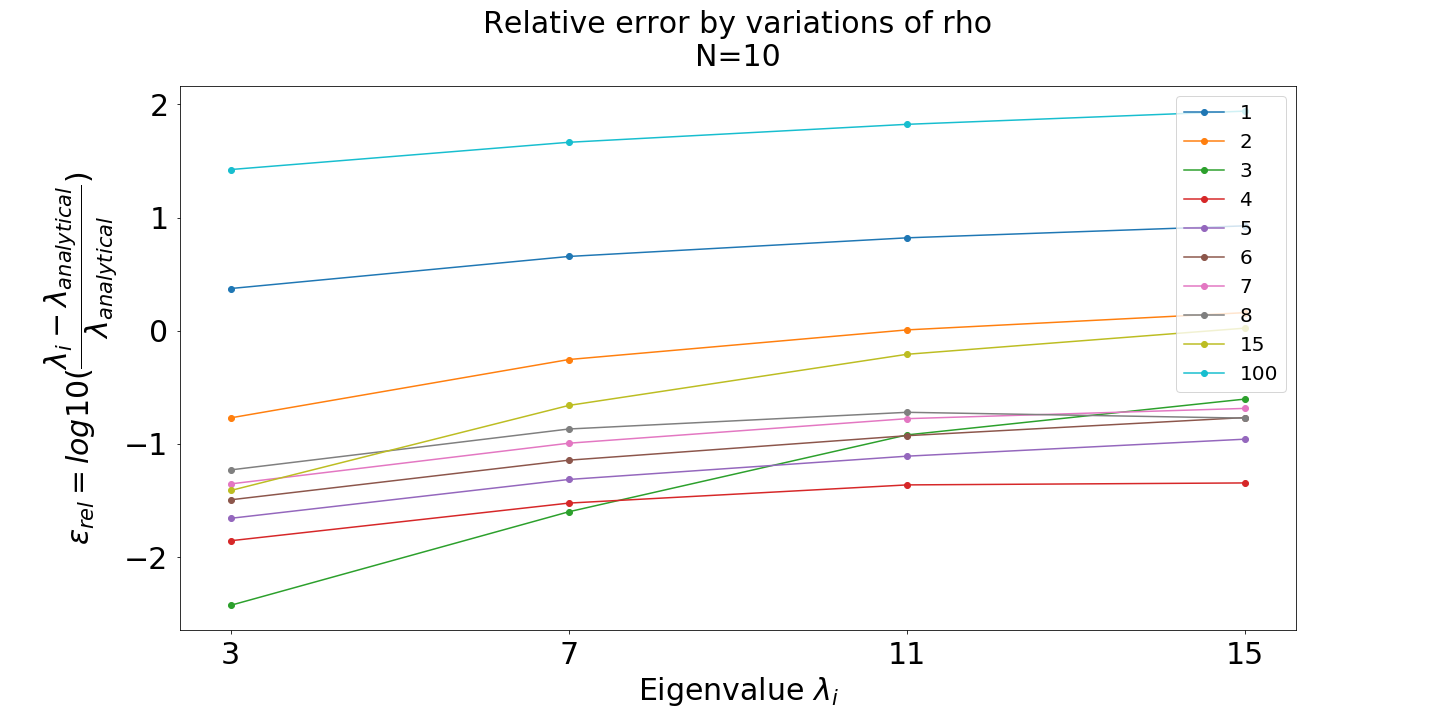
\includegraphics[scale = 0.21]{N_10_relative_error.png}}
	\subfloat{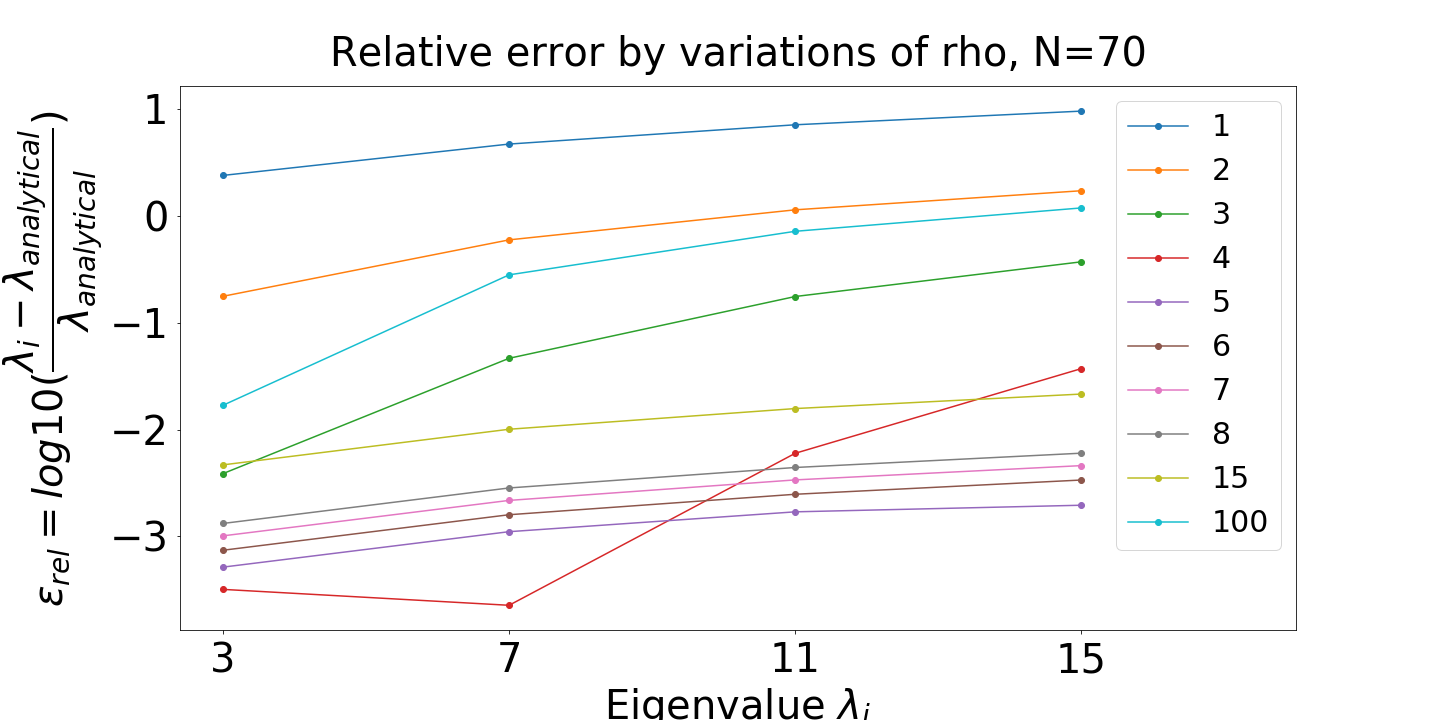
\includegraphics[scale = 0.21]{N_70_relative_error.png}} }
\end{figure*}
\begin{figure*}[!h]
	\noindent\makebox[\textwidth]{
		\centering 
	\subfloat{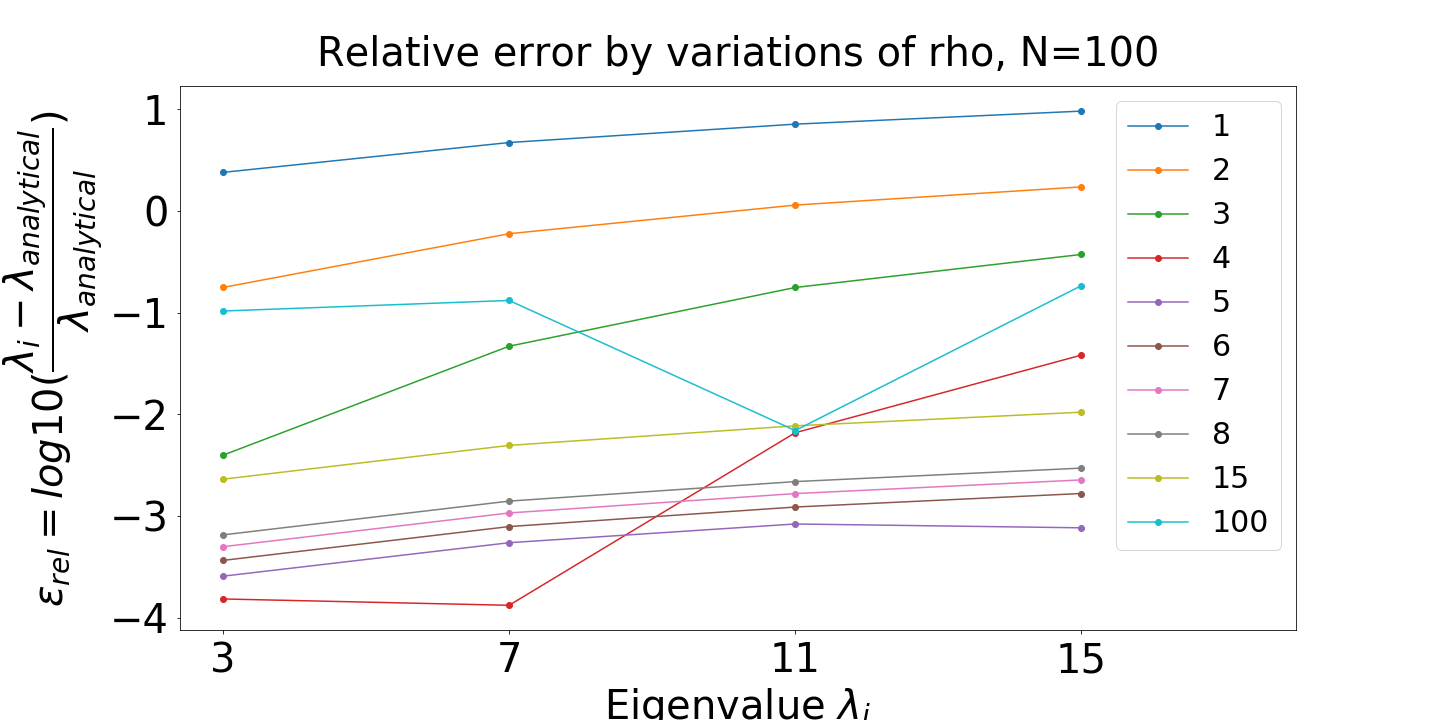
\includegraphics[scale = 0.21]{N_100_relative_error.png}}
	\subfloat{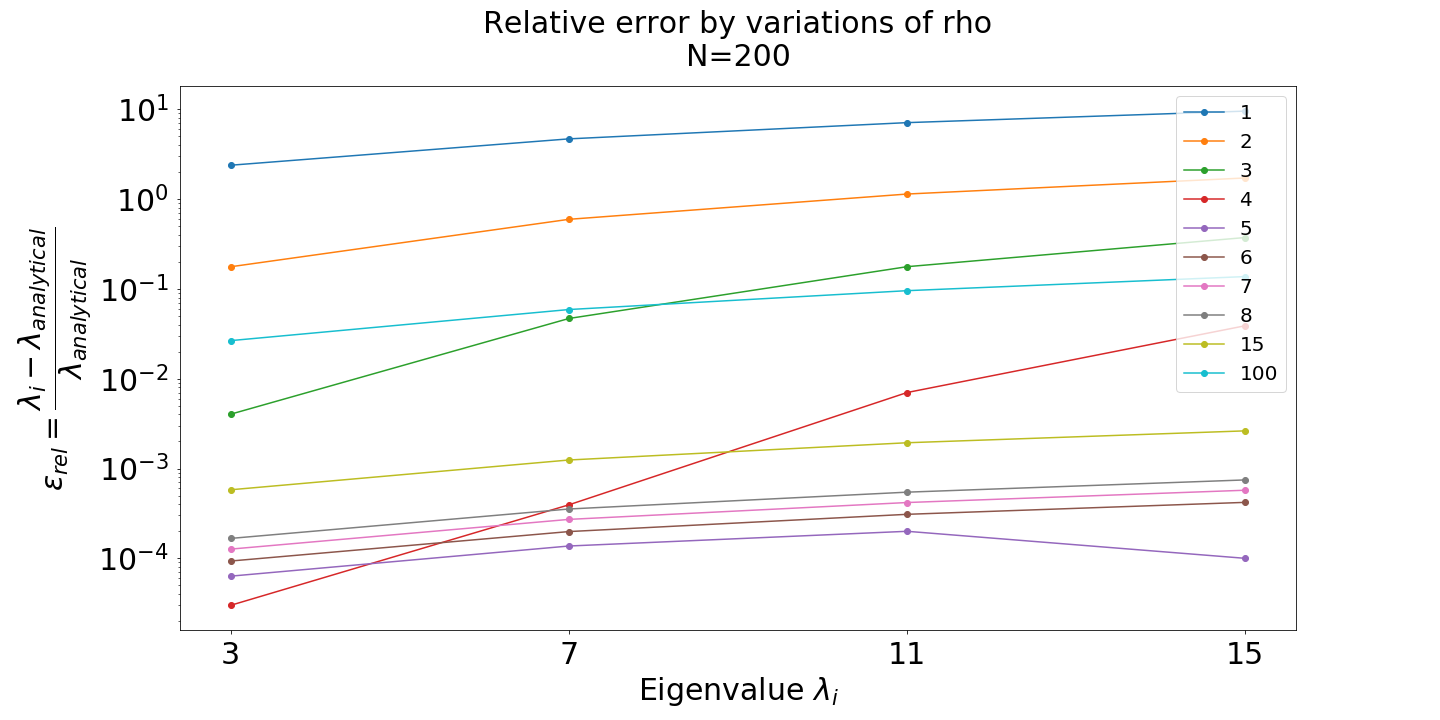
\includegraphics[scale = 0.21]{N_200_relative_error.png}}
	}
\caption{The relative errors between Jacobi's method and the analytical solution as a function of N and $\rho_{max}$. } \label{Nrho} 
\end{figure*}
\begin{figure*}[!h]
	\noindent\makebox[\textwidth]{
	\centering
	\subfloat{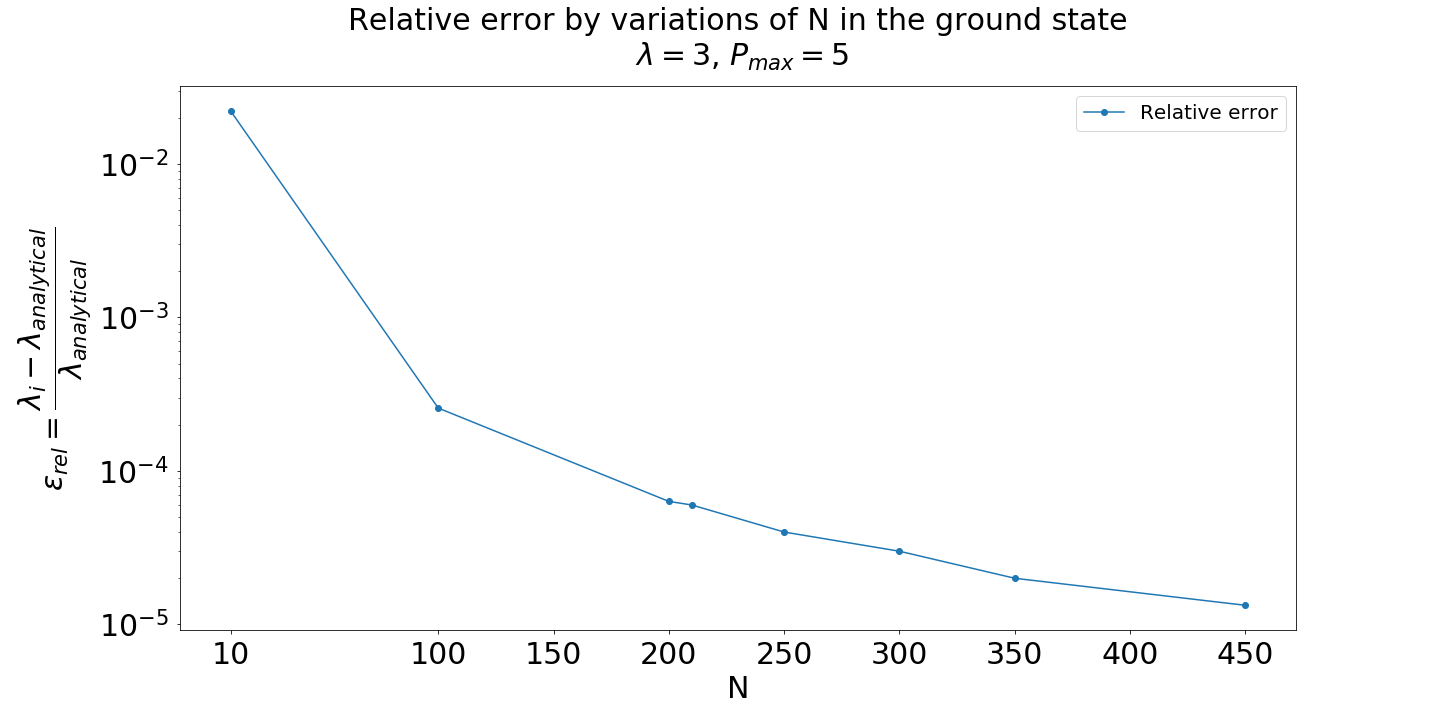
\includegraphics[scale = 0.21]{Relative_error_rho_5.png}}
	\subfloat{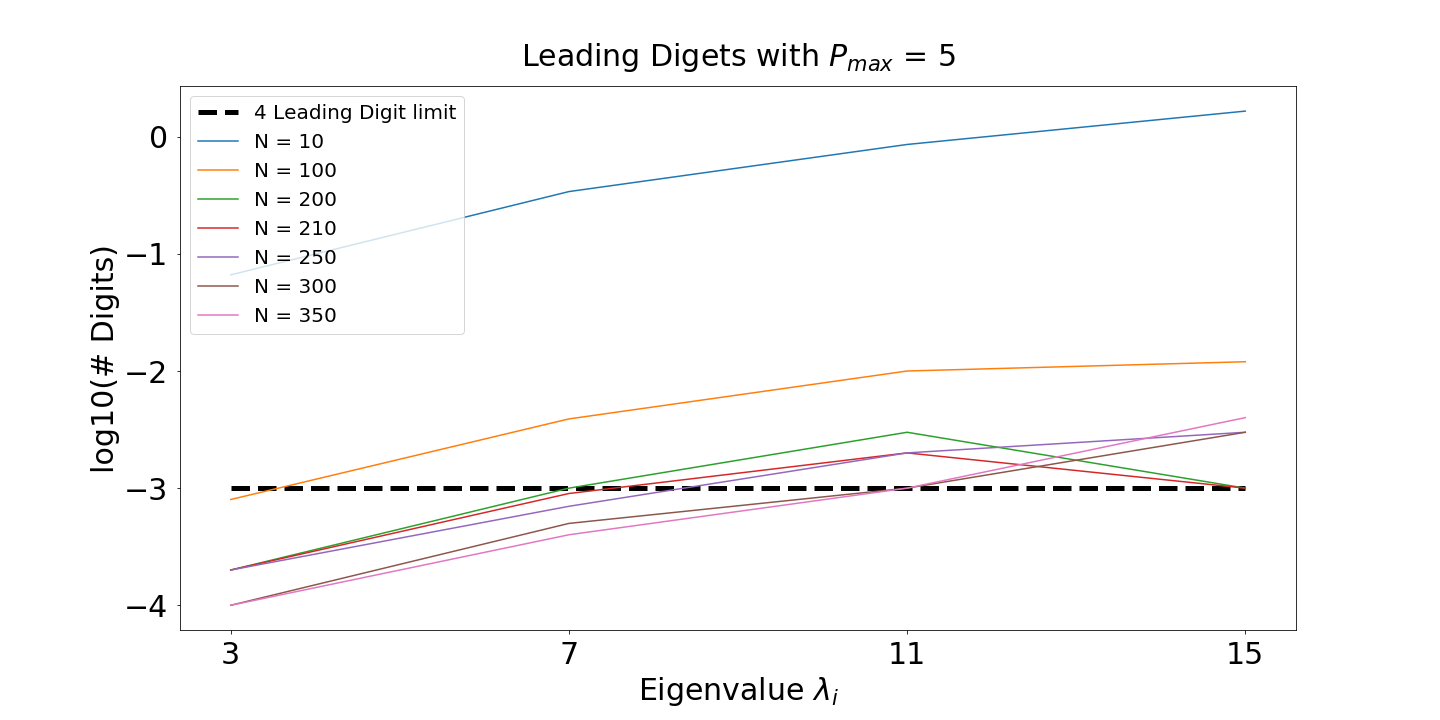
\includegraphics[scale = 0.21]{Leading_digits.png}} }
	\caption{The figure show the relation between the number for leading digits, in regards to the black bar representing four leading digits.} \label{fig:RE}
\end{figure*}
 
\subsection*{R\rom{3}. Quantum dots in three dimensions, two electrons} \noindent 
The ground state energy of a two-electron system as a function $\omega$ is presented in table \ref{tab2}. It is evident that the energy eigenvalue increases as $\omega_r$ increases. 

\begin{table}[H]
	\centering 
	\begin{tabular} {|c|c|}
		\hline
		$\mathbf{\omega}_r$ & $\mathbf{E(\lambda_0)}$\\ 
		\hline
		& \\ 
0.01 &  0.840704 \\
0.50 &  2.230826\\
1.00 &  4.057074\\
5.00 &  17.428622\\ 
\hline 
	\end{tabular}
	\captionof{table}[foo]{The energy eigenvalue for the ground state of a two-electron system in three dimensions. The value is an average of 10 independent calculations of the eigenvalue.\label{tab2}}
\end{table}

\subsection*{R\rom{4}. Quantum Physics Analysis of the result}\noindent 
The probability distribution with and without the repulsion between the two electrons are plotted in figure \ref{wavefunc} for the selected $\omega_r$ values. \\ \newpage 

\begin{figure*}
	\centering
	\subfloat{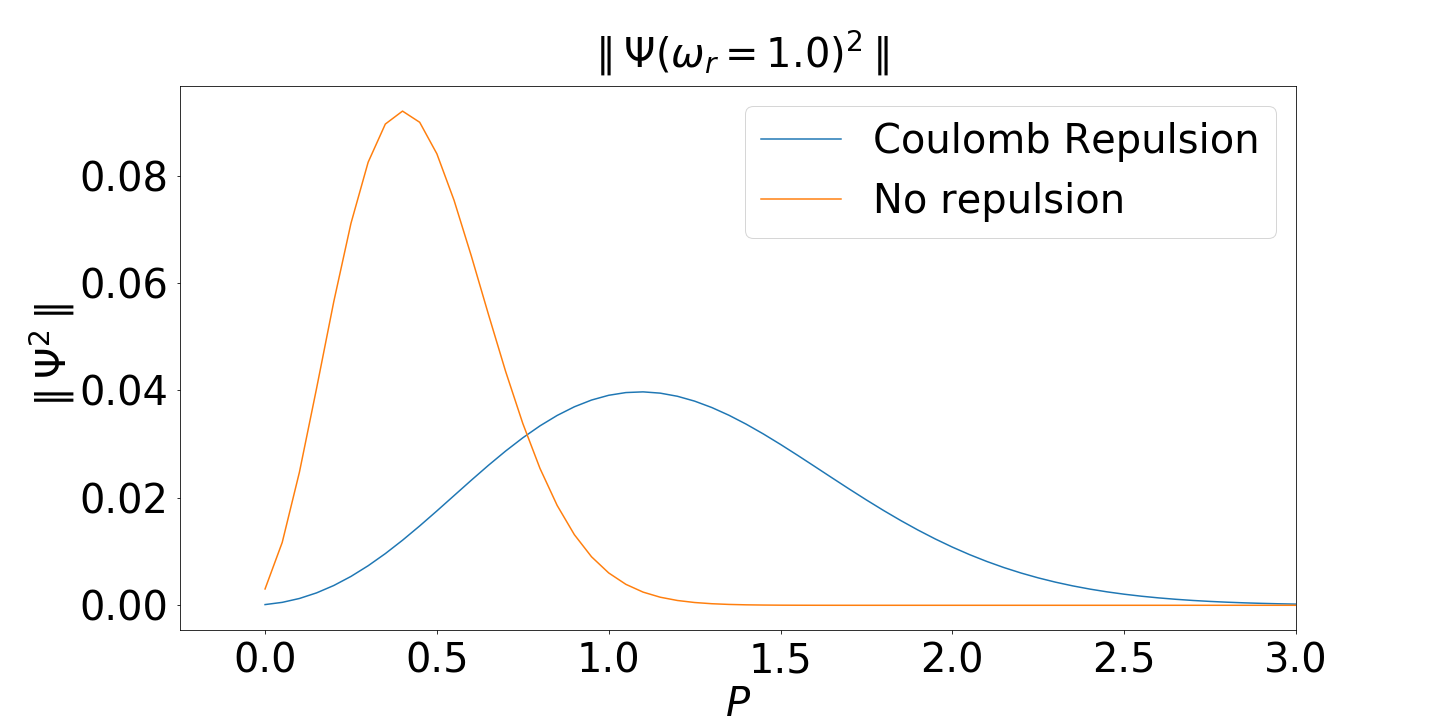
\includegraphics[scale = 0.18]{Omega_0_01.png}}
	\subfloat{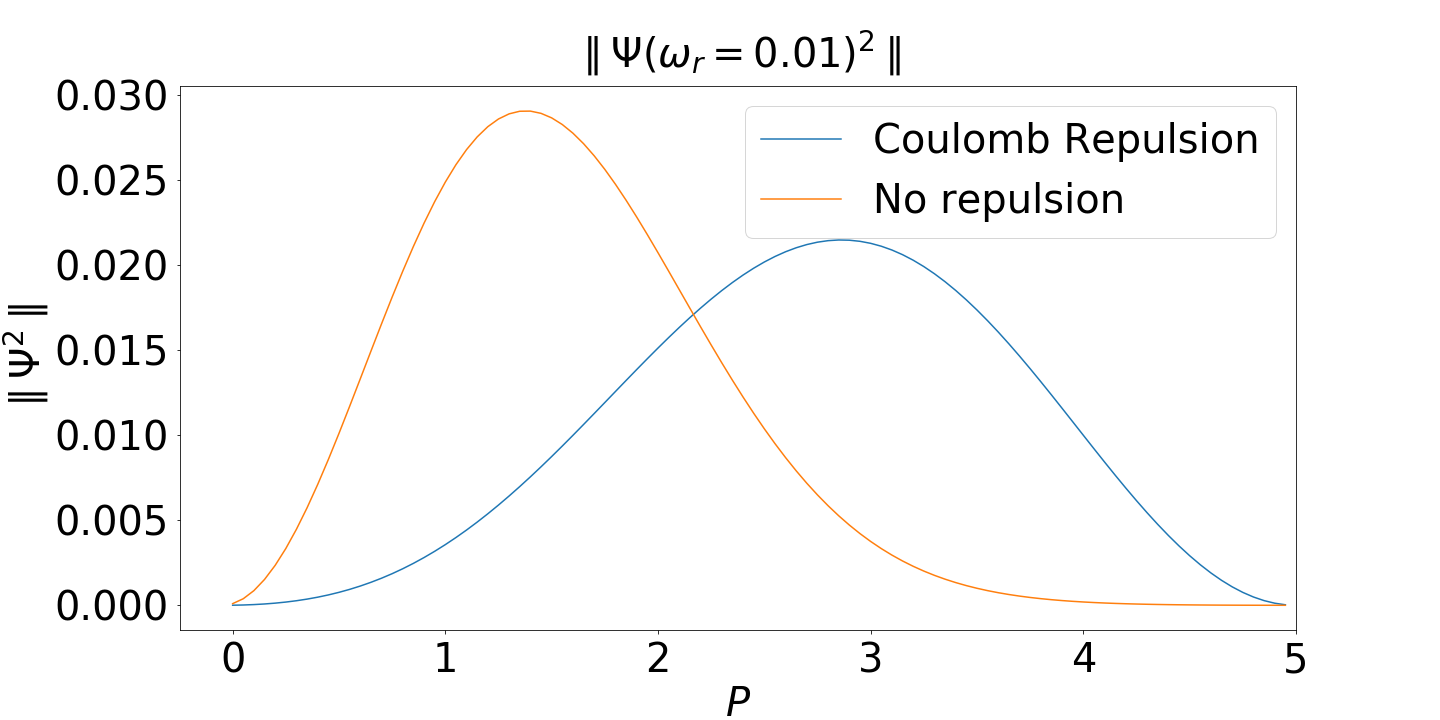
\includegraphics[scale = 0.18]{Omega_0_5.png}} \\ 
	
	\subfloat{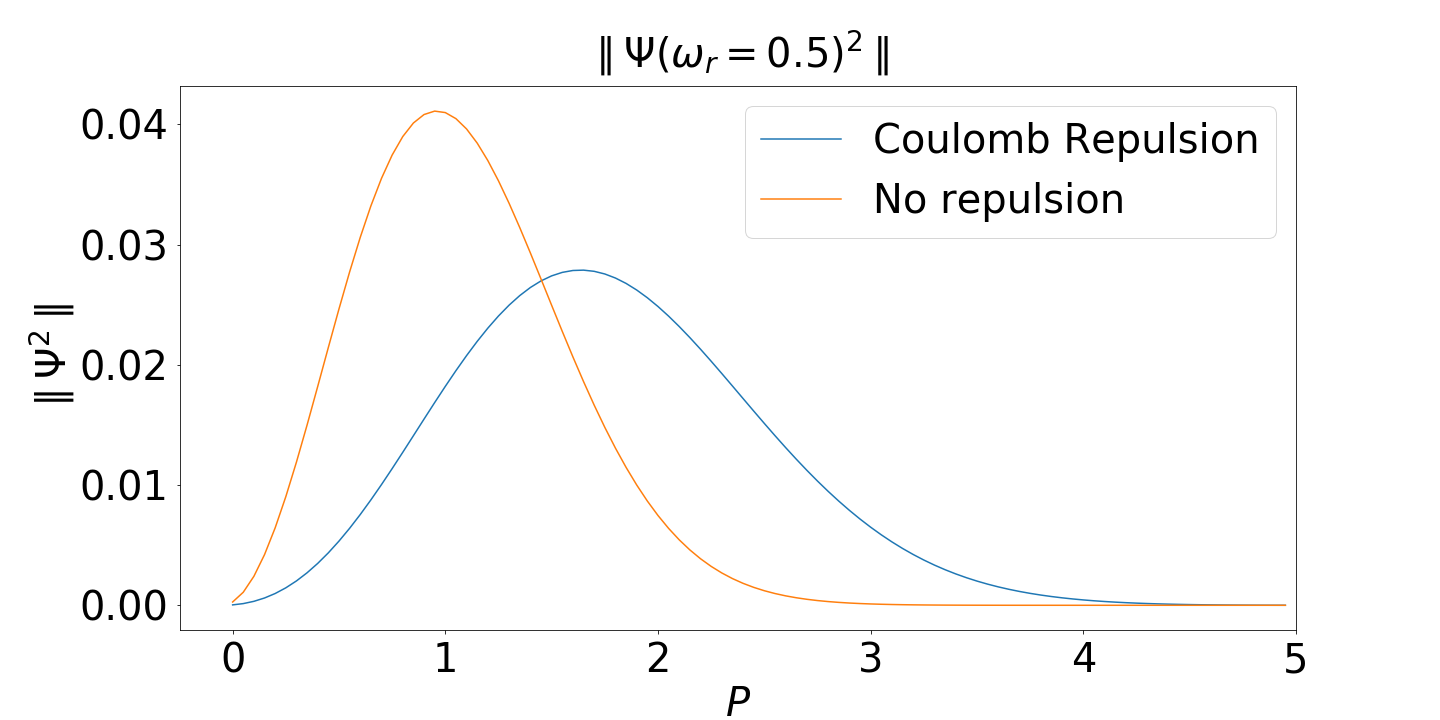
\includegraphics[scale = 0.18]{Omega_1_0.png}}
	\subfloat{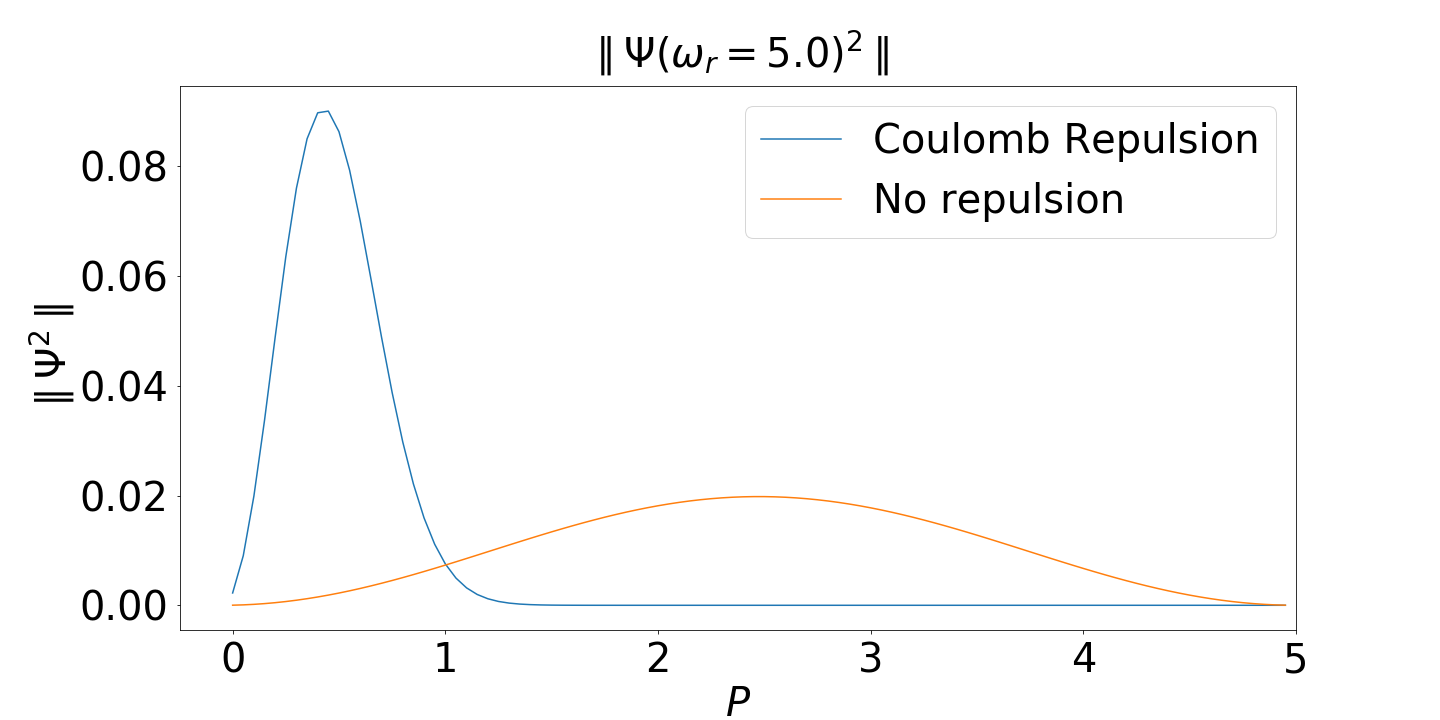
\includegraphics[scale = 0.18]{Omega_5_0.png}}
	\caption{The probability distribution with and without the repulsion between two electrons as a function of $\omega_r$} \label{wavefunc}
\end{figure*}

\section*{Discussion} 
\subsection*{D\rom{1}. The buckling beam}
We observe that Jacobi's method takes a lot longer than the Armadillo function, up to three orders of magnitude longer. It is well established that Jacobi's method is very inefficient for handling these kinds of tridiagonal systems. If we were to optimize the method further focusing on distinct properties of such a matrix, we might be able to reduce this time by a bit. \\ \indent 
It is also evident that the number of transformations needed to reduce the matrix to a diagonal form is the same every time we test the algorithm. This is a good indication that our method is stable, and does not alter the results significantly from time to time.  

\subsection*{D\rom{2}. Quantum dots in three dimensions for one electron} \noindent 
The relative error is observed to vary with each choice of N and $\rho_{max}$. It is evident that the error decreases as N increases, but furthermore, they all show the same tendencies in regards to $\rho_{max}$. $\rho_{max} = 5$ for all tested values of N appears to be the value that yields the lowest error for the ground state. One can observe some sort of distribution around $\rho_{max} = 5$, where the error increases as $\rho_{max}$ deviates further and further away from this value. For certain energy eigenvalues one can see $\rho_{max} = 3$ or $\rho_{max} = 4$ yielding lower relative errors also in the ground state. It is likely that access to a broader selection of analytical eigenvalues would help us determine the pattern indicated in this information. \\ \indent 
For one selection of $\rho_{max}$ it is possible to further investigate tshe trends in the relative error as a function of N. We did this for $\rho_{max} = 5$, and in figure \ref{fig:RE}.a we see a decay in the relative error with increasing N as previously indicated. This trend is not surprising, as one would typically expect a Toplitz matrix to have a relative error going like $\order{h^2}$. The function form of an error going as $\order{h^2}$ and our error-estimate appears to be the same. \\ \indent 
Furthermore, it is not surprising that the the number of grid points needed to reproduce the analytical results with four leading digests vary in regards to the energy eigenvalue. This is probably a property of the varying precision in the eigenvalue equation when solved in this discretized manner.  

\subsection*{D\rom{3}. Quantum dots in three dimensions for two electrons} \noindent 
It is not surprising that the energy eigenvalue increases as the strength of the oscillator potential increases. A higher potential strength will of course indicate a higher internal energy in the system for a given $r$.  


\section*{Conclusion}


\newpage .
\newpage 
\onecolumngrid
\section*{Bibliography}
\noindent $[1]$ Introduction to quantum mechanics, D.J. Griffiths and D. F. Schroter, 3rd edition, 2018, Cambridge University Press\\ 
$[2]$ Lecture notes 2015 for FYS3150, M. Jensen, 2015, university of Oslo
\section*{Appendix A}
For the code used for calculation our results, visit
\url{https://github.com/OlineRanum/FYS3150/Project_2}

\end{document}
